\documentclass[10pt]{article}
\usepackage[utf8]{inputenc}
\usepackage[T1]{fontenc}
\usepackage{amsmath}
\usepackage{amsfonts}
\usepackage{amssymb}
\usepackage[version=4]{mhchem}
\usepackage{stmaryrd}
\usepackage{graphicx}
\usepackage[export]{adjustbox}
\graphicspath{ {./images/} }
\usepackage{caption}
\usepackage{multirow}
\usepackage{hyperref}
\hypersetup{colorlinks=true, linkcolor=blue, filecolor=magenta, urlcolor=cyan,}
\urlstyle{same}

\title{Variable Impedance Actuators: a Review }

\author{B. Vanderborght ${ }^{6}$, A. Albu-Schaeffer ${ }^{1}$, A. Bicchi ${ }^{2,5}$, E. Burdet ${ }^{4}$, D.G. Caldwell ${ }^{5}$, R. Carloni ${ }^{3}$, M. Catalano ${ }^{2,5}$, O. Eiberger ${ }^{1}$, W. Friedl ${ }^{1}$, G. Ganesh ${ }^{4}$, M. Garabini ${ }^{2}$, M. Grebenstein ${ }^{1}$, G. Grioli ${ }^{2}$, S. Haddadin ${ }^{1}$,H. Hoppner ${ }^{1}$, A. Jafari ${ }^{5}$, M. Laffranchi ${ }^{5}$, D. Lefeber ${ }^{6}$, F. Petit ${ }^{1}$, S. Stramigioli ${ }^{3}$, N. Tsagarakis ${ }^{5}$, M. Van Damme ${ }^{6}$, R. Van Ham ${ }^{6}$, L.C. Visser ${ }^{3}$, S. Wolf ${ }^{1}$\\
${ }^{1}$ DLR/Institute of Robotics and Mechatronics, Germany, ${ }^{2}$ University of Pisa, Italy,\\
${ }^{3}$ University of Twente, Netherlands, ${ }^{4}$ Imperial College of Science, Technology and Medicine, United Kingdom, ${ }^{5}$ Istituto Italiano di Tecnologia, Italy, ${ }^{6}$ Vrije Universiteit Brussel, Belgium, http://www.viactors.eu corresponding author\\
bram.vanderborght@vub.ac.be}
\date{}


\begin{document}
\maketitle
\captionsetup{singlelinecheck=false}


\begin{abstract}
Variable Impedance Actuators (VIA) have received increasing attention in recent years as many novel applications involving interactions with an unknown and dynamic environment including humans require actuators with dynamics that are not well-achieved by classical stiff actuators. This paper presents an overview of the different VIAs developed and proposes a classification based on the principles through which the variable stiffness and damping are achieved. The main classes are active impedance by control, inherent compliance and damping actuators, inertial actuators, and combinations of them, which are then further divided into subclasses. This classification allows for designers of new devices to orientate and take inspiration and users of VIA's to be guided in the design and implementation process for their targeted application.
\end{abstract}

Keywords: Variable Impedance Actuators, Soft Robotics.

Actuators are key enabling components for motion generation and control with properties that greatly impact the overall performance of any mechanical systems. The lack of suitable actuators has hindered the development of high performance machines with capabilities comparable to humans, especially with respect to motion, safety and energy efficiency of human or other animals. The functional and neuro-mechanical control performances of bio-\\[0pt]
logical muscle far exceeds that of mechanical devices, with a key difference being the adaptable compliance or variable stiffness found in biological systems; this is very different from the performance of traditional stiff electrical drives used in industrial robotics, which require accurate, reference-trajectory tracking. Recent applications such as robots in close human/robot proximity, legged autonomous robots, and rehabilitation devices and prostheses, set different design specifications, where compliant actuators can have significant advantages over traditional actuation. Variable Impedance Actuators (VIA) are rapidly developing with a wide range of different actuators based on different principles, but as yet there is not "winning" design. Indeed, probably there is no winning actuator, but rather application dependent optimal solutions. To understand this "zoology", the VIACTORS consortium [1] provides in this paper an overview as well as a categorization, discussing advantages and disadvantages of the different designs. This work is the first of three papers on VIAs, which tries to organize the VIA state of the art, and establish a common language for designers and potential users of VIA technology. Grioli et al. [2] present a Variable Stiffness Actuator (VSA) datasheet as an interface language between designers and users and discuss design procedures and how data generic VSA data may be organized to minimize the engineer's effort in choosing the actuator type and size. Wolf et al. [3] propose VSA Design Guidelines for R\&D engineers facing the challenge of designing new VSA systems and implementing them in use-cases as shock absorbing, stiffness variation, cyclic motions and explosive motions. The development and exploitation of novel actuation technologies will create a new generation of robots that can co-exist and co-operate with people and get much closer to the human levels of manipulation, locomotion and rehabilitation performances.

\section*{1. What is a Variable Impedance Actuator?}
To define what a Variable Impedance Actuator (VIA) is, it is useful to start by defining a non-VIA (traditional stiff) actuator. A stiff actuator is a device, able to move to a specific position or track a predefined trajectory. Once a position is reached, the actuator will hold this position, (ideally) whatever the external forces (within the force limits of the device). It is a position source, i.e. a system with a very high (ideally infinite) mechanical impedance. This behavior is obtained when a motor has a high gear ratio (eg servomotors) aiming to be as stiff as possible [4]. Such actuators have\\[0pt]
excellent trajectory tracking with a high bandwidth and high accuracy. They are common in industrial robots. A VIA in contrast deviates from its set equilibrium position, depending on the external forces and the mechanical properties of the actuator (mostly inertia, stiffness and damping factors). Equilibrium is defined as the position where the actuator generates zero force or torque (also called virtual position by Hogan [5]). This concept is specific to VIA actuators, since it does not exist for stiff actuators. An extreme case is where the impedance is zero and the actuator forms a force/torque source or transparent actuator, eg gravity is a force source. Examples where a force/torque source are approached are direct drive motors [6] or constant torque springs.

VIAs are important in Embodied Intelligence. Pfeifer and Bongard [7] state that adaptive behavior is not just control and computation, but it emerges from the complex and dynamic interaction between the robot's morphology, sensory-motor control, and environment. Through smart design of the body and the actuators part of the computational intelligence can be outsourced to the embodied intelligence making many tasks become simpler.

Position control in a task in which a robot interacts with the environment, is not a properly posed problem because the controller is dependent on parameters, which are out of the control potential [8] [9]. Yet, controlling the impedance and the equilibrium position is a well-posed problem that is independent of the knowledge of the environment, if within certain boundaries. Applications of VIA are consequently found were robots must physically interact with an unknown and dynamic environment and the control body-actuator system must have abilities like [10]:

\begin{itemize}
  \item Efficiency e.g. natural gait generation, adaptation in legged locomotion and prosthetics for lower limbs, explosive motions such as throwing or kicking;
  \item Robustness to external perturbations and unpredictable model errors (changes) of the environment, of the robot kinematics and dynamics, or of the dynamics of a human interacting with it;
  \item Adaptability and force accuracy in the interaction with the operator, in applications in which continuous contact and accurate force exchange is necessary, such as in "hands-on" assistive devices, rehabilitation, exoskeletons and haptics;
\end{itemize}

\begin{figure}[h]
\begin{center}
  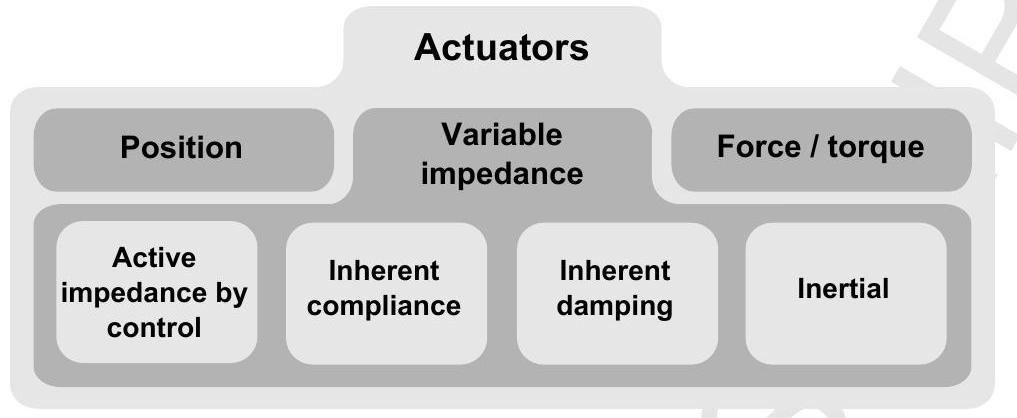
\includegraphics[width=\textwidth]{2025_09_17_f0417c8723605e4ad1efg-04}
\captionsetup{labelformat=empty}
\caption{Figure 1: Main categorization of actuators.}
\end{center}
\end{figure}

\begin{itemize}
  \item Safety to humans (and resilience to self-damage) in operations where the robot has fast, accurate motions, while cooperating, physically interacting or even possibly colliding with the humans and their environment, including other robots.
\end{itemize}

Variable Impedance Actuators will be categorized depending on how their stiffness and damping can be achieved, Fig. 1. This is a revision of the work by Van Ham et al. [11]. A first division can be made between active impedance by control, inherent compliance and damping actuators, inertial and a combination of them.

In this section the terms impedance, admittance, compliance, stiffness and damping are introduced and a relationship between them is provided. Mechanical interaction between two systems A and B can be modeled looking at the dynamic relation between the variables which characterise the energy exchange and interaction behaviour between the two systems. The resulting interaction force and motion between A and B cannot be attributed solely to one of the systems but is the combination of an intrinsic property (behaviour) of A and an intrinsic property (behaviour) of B . These intrinsic behaviours are referred to as impedance and admittance. If the system $A$ is modelled as an impedance, system B must be modelled as an admittance to complement the other. A mechanical impedance is a dynamic relation which generates a force (in time) as a function of a displacement (in time). This differential relation can be linear (modellable usually with Laplace methods) or non linear (modellable with nonlinear functional analysis tools, such as e.g. jet bundles). Admittance is the complement of impedance. Stiffness is the differential relation between infinitesimal differences in force and po-\\
sition. Compliance is the inverse. Stiffness and compliance are related to elastic energy storage. Damping is a differential relation between infinitesimal changes in force and velocity, and is related to irreversible transduction of mechanical energy to heat and as such takes energy out of the systems.

\section*{2. Active impedance by control}
Active impedance by control is when an actuator mimics the impedance behavior using software control [12]. Based on the measured output state, a correction is calculated by the controller and set by the (stiff) actuator. This type of VIA has an actuator, sensor and controller that are fast enough for the application, but no energy can be stored and due to the limited bandwidth of the controller no shock can be absorbed (e.g. hitting with a bat will not be handled by the system with the desired impedance setting). Similarly, exploiting energy efficient natural dynamics (cf passive walkers [13]), is not possible since energy is required to move. Also the impedance controller is quite complex and requires accurate system dynamics models. An advantage of controlled impedance is that it can adapt both the damping and stiffness (contributing to the impedance of the system) online and this in a theoretical infinite range and with infinite speed. This technique pioneered by DLR and commercialized by Kuka is now considered mature [14]. Active impedance control has been shown in hydraulic actuators on systems such as the quadruped HyQ [15] and Sarcos [16]. Fasse et al. [17] present an active controlled impedance where 3 currents are controlled on the 2 or more available independent windings in the stator or rotor of an electromagnetic motor. This differs from the state feedback strategies described above as the control of torque, stiffness and damping is independent of the feedback from the output, ensuring passivity.

\section*{3. Inherent compliance}
In contrast to active impedance by control, passive compliance contains a passive or intrinsic compliant element. This category can sub-divided into mechanisms where the compliant element cannot change its stiffness (fixed compliance) with the variable impedance created by software control, and adaptable compliance systems where the stiffness is controlled by mechanical reconfiguration. The advantage here is that the very high (virtually infinite) bandwidth for the passive compliance can absorb impact shocks and store\\[0pt]
energy. Usually the design is more complex with more components than for the controlled impedance. Such systems typically have a very low intrinsic damping for efficient energy storage and retrieval, this means that the desired damping behavior for task execution must be implemented in control [18] or using an additional inherent damping device (see Section 4).

\subsection*{3.1. Fixed compliance properties}
The most famous inherently compliant actuator is the original Series Elastic Actuator (SEA) [19], which is a spring in series with a stiff actuator. The actuator stiffness is fixed and determined by the spring selection, thus the physical stiffness cannot be changed during operation. Sugar [20] developed a spring-based actuator, using the concept of equilibrium controlled stiffness, in which, a linear spring is series to a stiff actuator and the spring equilibrium position is controlled to exert a desired force or stiffness. The stiffness is actively changed using a control law rather than by passively adding springs. The force control problem becomes a position control problem using electric motors. The motor position is adjusted based on the deflection of the spring to alter the tension or compression of the spring. Tsagarakis et al. [21] developed a ComPact ${ }^{\text {© }}$ soft actuator for the iCub robot using 6 linear springs for the compliant element sandwiched between the three spoke structure of the motor side reduction drive and the three spokes of the output link. The velocity based controller generates velocity commands that are a function of the desired virtual stiffness using the spring deflection state. In the Distributed Elastically Coupled Macro Mini Actuation (DECMMA) approach [22], a SEA is placed in parallel with a second smaller motor to recover control bandwidth in the high-frequencies, later called Distributed Macro-Mini Actuator-DM ${ }^{2}$ [23] for an antagonistic setup.

\subsection*{3.1.1. Nonlinear SEA}
As nonlinear stiffness seems to be advantageous for tasks such as jumping and hopping [24], the HypoSEA [25] was designed to use a hypocycloid mechanism to stretch a linear spring in a nonlinear way. For safety the safe link mechanism (SLM) by Park et al. [26] maintains very high stiffness up to the pre-determined critical impact force, but provides very low stiffness above this value, thus absorbing the impact acting on the robot arm. The critical impact force is set by adjusting the initial transmission angle of the double-slider mechanism, the spring constant and the initial spring length. In the V2E2 actuator [27] energy efficiency is achieved by combining an Infinite

Variable Transmission (IVT) and an elastic element. The spring element is used to store mechanical energy where any force profile can be achieved by changing the transmission ratio of the IVT. Energy can be injected in the system by a motor-clutch mechanism making it very suitable for cyclic motions like walking or to compensate different constant loads at zero energetic cost. Since the actuator has only one control parameter (the transmission ratio), the torque and stiffness are coupled.

\subsection*{3.2. Adaptable compliance properties}
Several groups have designed adaptable compliance mechanisms, with elastic elements storing energy, in addition to altering the stiffness. This concept gives intrinsic capabilities (bandwidth, impacts, energy storage) over the joint stiffness range. However, two motors are required: one to control the equilibrium position and the second to control stiffness. In this section, a classification is presented, based on the main principle on which the adaptive stiffness is obtained (see Fig. 2). The different actuators from literature can be classified into three major groups:

\begin{itemize}
  \item Spring Preload: Stiffness is altered by changing the spring preload.
  \item Changing transmission between load and spring: The stiffness is altered by changing the transmission ratio between the output link and the elastic elements.
  \item Physical properties of the spring: The physical structure of the spring itself is altered.
\end{itemize}

Some devices use combinations of these main three mechanical properties.

\subsection*{3.3. Spring preload}
In the Spring Preload category the stiffness is adjusted by changing the pretension or preload on the spring. Compared to the no load category, the spring force is parallel to the spring displacement, hence to change the stiffness, energy has to be stored in the springs and may not be retrievable. To overcome this a second spring with negative stiffness can be added, usually resulting in a large passive angular deflection. This class can be further divided in the following subclasses:

\begin{figure}[h]
\begin{center}
  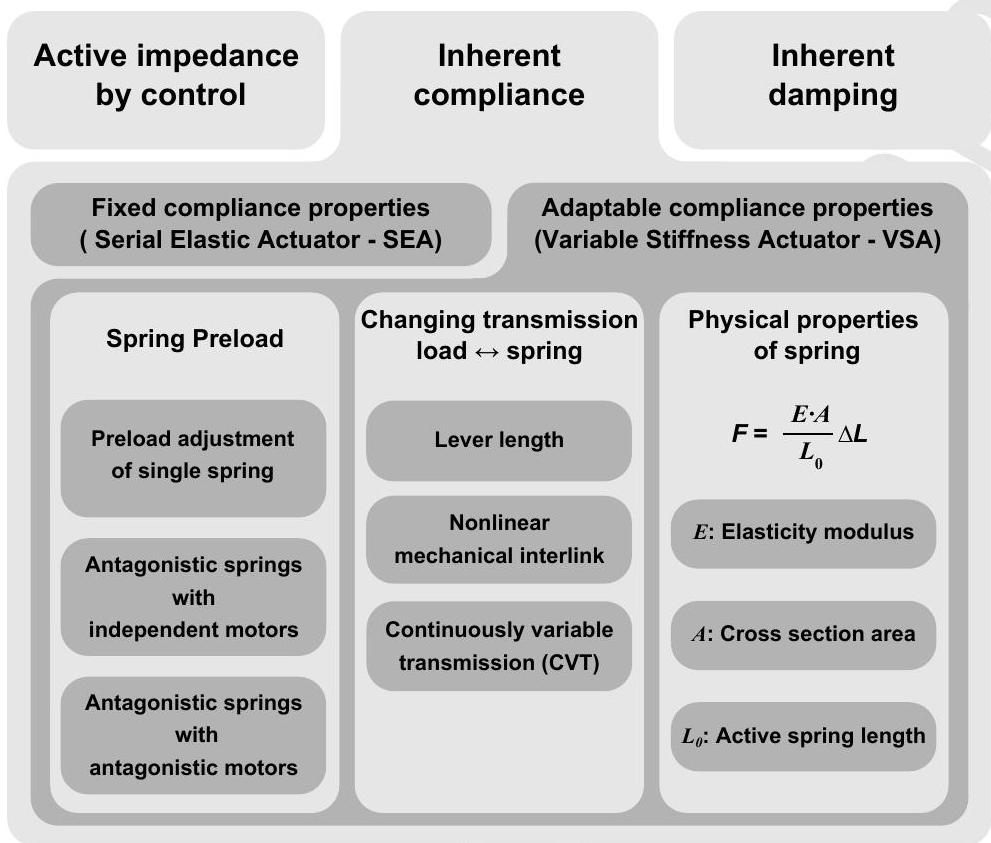
\includegraphics[width=\textwidth]{2025_09_17_f0417c8723605e4ad1efg-08}
\captionsetup{labelformat=empty}
\caption{Figure 2: Overview of passive compliant actuators.}
\end{center}
\end{figure}

\begin{itemize}
  \item Antagonistic Springs with Antagonistic Motors: Both the springs and the motors are placed in an antagonistic setup where at least two nonlinear springs are required. To change the stiffness both motors have to move in opposite direction to preload the springs, to change the equilibrium position both motors have to work in the same direction.
  \item Antagonistic Springs with Independent Motors: Similar to the first class, except that the motors (partly) decouple the equilibrium position and stiffness control.
  \item Preload Adjustment of Single Spring: This class is not antagonistic, 1 linear spring is enough and the preload is changed by a motor to control the stiffness. A second motor controls the equilibrium position.
\end{itemize}

\subsection*{3.3.1. Antagonistic Springs with Antagonistic Motors}
Agonist/antagonist actuator pairs are common in nature [28] and robotics. Rotation of the actuators in the same sense generates a net joint torque, while\\[0pt]
counter-rotation sets different levels of effective joint stiffness. Although agonistic-antagonistic actuation for variable stiffness is well known, it is useful to recall the three different possible embodiments (see Fig. 3). These will be referred to as "uni-directional", "cross-coupled", and "bi-directional" antagonistic arrangements. When tension-only tendons are considered for the uni-directional case [29], the maximum joint torque can not be more than that of each single motor, and no net torque is available when stiffness is at maximum. To overcome these limitations, a third compliant element (possibly different from the two antagonists) may be introduced to cross-couple the two prime movers (see Fig. 3-b). Cross-coupling allows setting of preload forces to tune it to nominal working conditions, using (a fraction of) each motor's torque in both directions. The VSA-I prototype is an example of a such a cross-coupled device [30]. One further step introduces a fourth spring to connect each actuator to the link via two compliant elements (not necessarily symmetric) in push-pull configuration (see Fig. 3-c). This configuration is used in the VSA-II prototype [31], the VSA-cube that is a hobby servomotor style of VIA actuator [32] and in the VSJ [33], used to actuate the wrist and forearm of the DLR hand/arm [34]. The big advantage here is that the sum of the two motor torques are available at the joint side if you drop the requirement to track a desired stiffness. The passive joint range of a setup of antagonistic springs is that both the angular and passive joint ranges are limited to the maximum extension of the springs. An interesting approach to reduce the energy consumption of an active knee prosthesis was introduced in [35], where during the walking cycle of the knee, not always both springs were engaged due to a clutch mechanism. Most of the VIAs are powered by electromagnetic motors, but also other means are possible like the hydraulic pistons used in an antagonistic setup for the NEUROexos elbow exoskeleton [36] or pneumatics [29] [37].

\subsection*{3.3.2. Antagonistic Springs with Independent Motors.}
The main disadvantage of using antagonistic motors is that both motors need to work synchronously to either change the equilibrium position or the stiffness. This means the motors cannot be dimensioned for a specific task. For Antagonistic Springs with Independent Motors, the motors are arranged to (partially) decouple the control of equilibrium position and stiffness 4.

For the Quasi-Antagonistic Joint (QA-Joint) [38] one motor (the link drive) adjusts the link side position, while the second motor (the stiffness drive) operates the stiffness adjustment. This is a partially decoupled system

\begin{figure}[h]
\begin{center}
  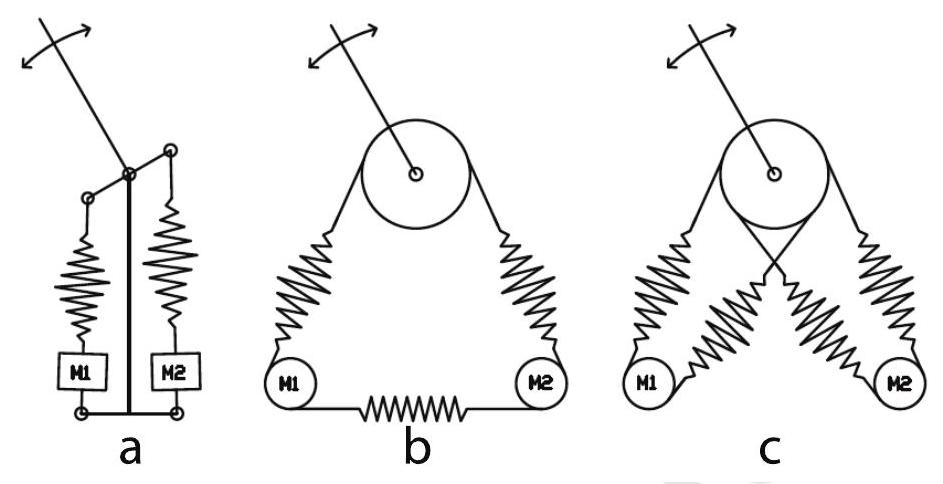
\includegraphics[width=\textwidth]{2025_09_17_f0417c8723605e4ad1efg-10}
\captionsetup{labelformat=empty}
\caption{Figure 3: Possibilities in Antagonistic Springs with Antagonistic Motors: "uni-directional", "cross-coupled", and "bi-directional" antagonistic arrangements.}
\end{center}
\end{figure}

since when the stiffness is changed, the equilibrium position must be adjusted by the link side motor. Complete decoupling of the equilibrium position setting and the stiffness occurs when the endpoints of the two springs are mechanically coupled either by a lever arm or a pulley like e.g. the AMASC actuator [39]. Here the motor to set the equilibrium position is not on the joint but on the other side of the nonlinear springs. It is also possible to move this motor to the joint, making the design less complex. In this case the equilibrium position of both lever arms is horizontal, and the motor for the equilibrium position of the actual joint sets the relative position of the arm of the joint with respect to the lever arms [40]. With this design the angular joint range is extended, since it is not limited to the maximum extension of the springs.

\subsection*{3.3.3. Producing nonlinear springs}
To obtain adaptable stiffness in an antagonistic setup, the springs need to be nonlinear [11] with a quadratic force-length function forming the most common tendon elastic characteristics [41]. This design (with two identical antagonistic springs) results in a constant joint stiffness characteristic, independent of the joint angle deflection. Also rubbers and polymers are non-hookean and can be shaped to create nonlinear elastic behavior. Fig. 5 presents some possibilities.

A first option is to use variable pitch progressive springs where each coil is spaced differently with a variable spring rate (Fig. 5a). The different coils

\begin{figure}[h]
\begin{center}
  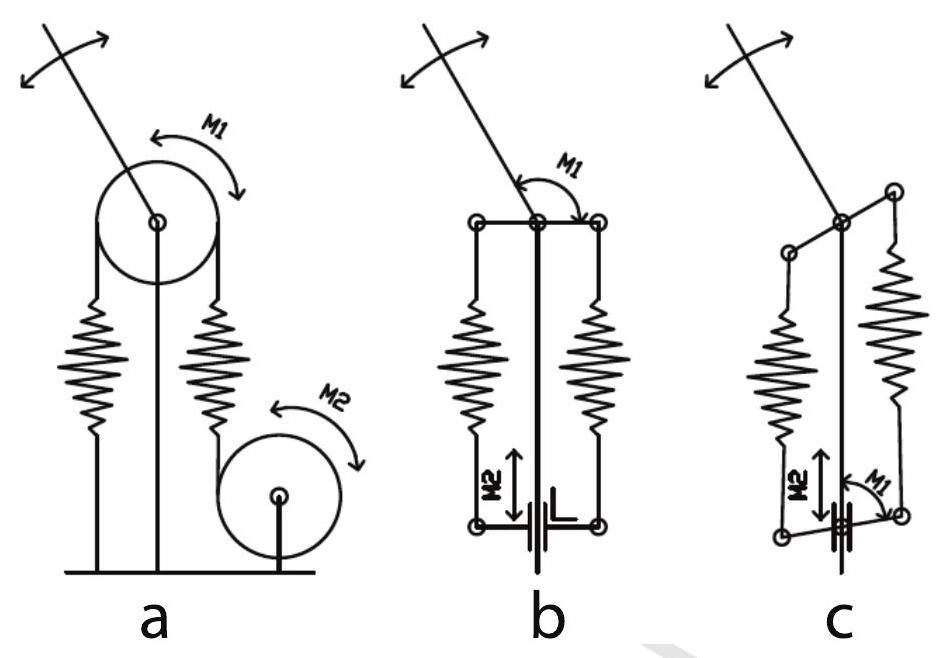
\includegraphics[width=\textwidth]{2025_09_17_f0417c8723605e4ad1efg-11}
\captionsetup{labelformat=empty}
\caption{Figure 4: The different possibilities in the class Antagonistic Springs with Independent Motors.}
\end{center}
\end{figure}

are achieved with variable pitch, conical or mixed. When free, the spring initially is easily compressed, however, as more forces are applied, the coils on a progressive spring come closer and at a certain point, coils at the top $1 / 4$ touch, finally becoming inactive, and that makes the spring stiffer.

Tonietti et al. [30] describe the Variable Stiffness Actuator (VSA) where the nonlinearity is created by a linear spring pushing the tendon into a triangle (Fig. 5b). The height of this triangle relative to half base determines the stiffness of the mechanism. Disadvantages are the limited life cycle and load capacity of the timing belt. This mechanism has been used in a simplified form in [42] (Fig. 5c). To further simplify the design one pulley can act as the mechanism winder as seen in the DLR hand/arm system [43].

Others, such as Migliore et al. [44] use shaped pieces, over which two wheels roll to transform the characteristic in a nonlinear shape (see Fig. $5 \mathrm{~d})$. The centers of the wheels are interconnected by a linear spring. With this design the spring force-elongation characteristic can be chosen during the design phase, as well as the resulting compliance characteristic of the overall system. The drawback is the size, extra complexity, and friction in the quadratic spring mechanism. The QA joint uses a cam profile with rollers to implement a rotational setup [38].

The VSA-II [31] and VSA-HD [32] have a four-bar mechanism, which\\[0pt]
is a special case of Grashof four-bar linkage (Grashof neutral linkage), Fig. 5e. By appropriate link lengths selection the nonlinear relationship between input and output link angles can be regulated. Huang et al. [44] used an antagonistic pair of four-bar linkages where the linear spring is placed between two opposing nodes and the nonlinear output force is obtained from the two other nodes.

Pneumatic designs such as Pneumatic Artificial Muscles (PAM's), with the McKibben muscles the most well-known, which when pressurized, contract axially while expanding radially can also be used (Fig. 5f) [45] [37]. Here air compressibility makes them inherently compliant and spring-like, however, braid friction can cause hysteresis problems and dead bands making them difficult to control. The Pleated Pneumatic Artificial Muscle (PPAM, [29] [46]) reduces hysteresis and overcomes the threshold of pressure (deadband). Pneumatic muscles have a high power to weight ratio and can be directly coupled to the joint without gearing, but each joint needs two actuators and the resultant characteristic can be highly nonlinear. The drawbacks of a joint actuated by two pneumatic muscles are the nonlinear characteristic, the slow dynamics (especially depressurizing the muscle is slow), the presence of hysteresis, and the need for pressurized air.

Electroactive Polymers (EAPs) are another candidate technology that produce large deformations under an external electric field and they have the necessary nonlinear stress-strain relationship. Randazzo et al. [47] working on a rotational joint driven by two antagonistic Dielectric Elastomer Actuators (DEA) showed that the joint stiffness change is small. DEAs are superior to traditional electromagnetic actuators in terms of weight and energy efficiency, but they are still slower, produce low forces and require high voltages to operate [48].

This subclass uses nonlinear springs, which is often a drawback, but the antagonistic springs also reduce energy efficiency and energy storage capacity. Hurst and Rizzi [39] abandoned the antagonistic setup in Mabel calculating that this significantly reduced energy storage capacity as energy must transferred from one spring to another rather than directly to the joint. Another study [49] described how an antagonistic setup using two SEA consumes more energy for a certain motion compared to a Maccepa actuator (The Mechanically Adjustable Compliance and Controllable Equilibrium Position Actuator). Carloni et al. [50] developed a metric for comparing the energy efficiency of VSA designs with results in accordance with [49].

\begin{figure}[h]
\begin{center}
  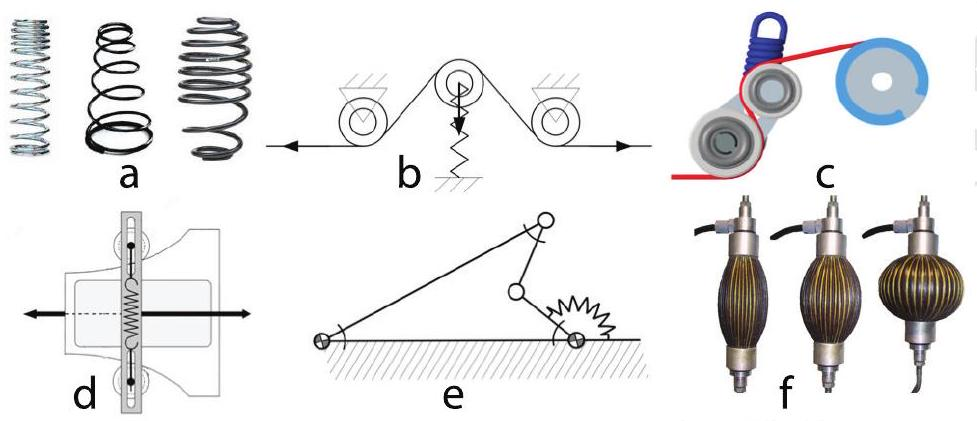
\includegraphics[width=\textwidth]{2025_09_17_f0417c8723605e4ad1efg-13}
\captionsetup{labelformat=empty}
\caption{Figure 5: Different possibilities of nonlinear springs (a) progressive springs, b) triangle mechanism, c) adapted triangle mechanism, d) cam mechanism, e) four-bar mechanism, f) pneumatic muscles.}
\end{center}
\end{figure}

\subsection*{3.3.4. Preload Adjustment of Single Spring}
The main feature of this subclass is the use of a nonlinear connector between the output link and the spring element hence only one linear spring is required. The stiffness adjustment is however still performed by changing the preload on this single spring.

In the Maccepa [51] (see Fig. 6a), the position of a lever arm is controlled to set the equilibrium position. The lever arm is connected to a spring loaded pivot point on the output link via a wire. When the link is moved out of the equilibrium position, the spring extends forcing the joint back to the equilibrium position. By pretensioning the spring different stiffness setting can be achieved. The MARIONET (Moment arm Adjustment for Remote Induction Of Net Effective Torque) [52], replaces the pretensioned spring with a tensioning motor. In the Maccepa 2.0 [67] (Fig. 6b) the lever arm is replaced by a cam so the torque angle and stiffness-angle relation can be chosen depending on the application. The Maccepa can be built with off-the-shelf components and has a linear angle-torque characteristic, making it readily suitable for different applications [53] [54].

The VS-joint [33] (Fig. 6c) can be seen as the complement of the Maccepa. In this case a preload is responsible for the change of stiffness rather than a pretension. A roller is pushed by a spring to the lowest position in the cam disk which is the equilibrium position. When a torque is applied to the joint, there will be a joint deflection of the roller and pushing the roller upward causing a translational deflection of the springs. The spring pushes the roller downwards, which will generate a force in the direction of the lowest point of

\begin{figure}[h]
\begin{center}
  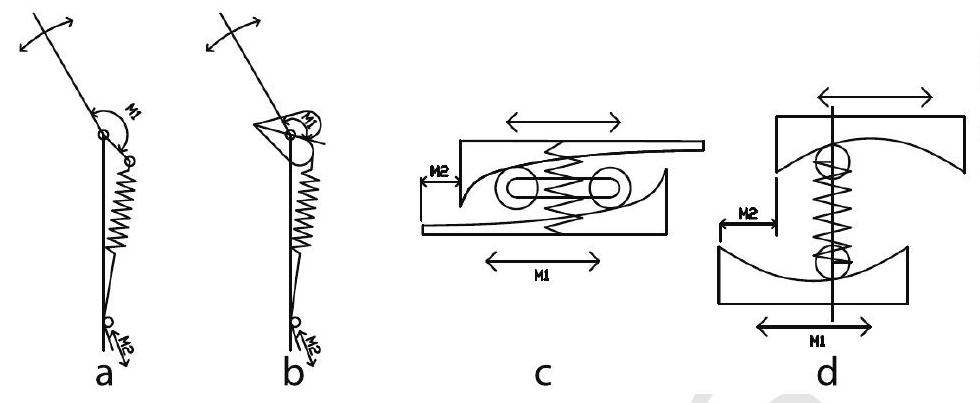
\includegraphics[width=\textwidth]{2025_09_17_f0417c8723605e4ad1efg-14}
\captionsetup{labelformat=empty}
\caption{Figure 6: The possibilities in the class Preload Adjustment of Single Spring (a) Maccepa, b) Maccea 2.0, c) VS joint, d) FSJ. )}
\end{center}
\end{figure}

the cam disk. The advantage of this design is that it can easily be integrated into a robotic arm. The shape of the cam disk can be adjusted to obtain a progressive, regressive, or linear system behavior. Although one spring is enough, the VS joint uses three springs for symmetry. Both designs allow that two motors of different sizes can be used: a small one for the stiffness preset and a more powerful motor for the link position.

In contrast to the mechanics of the VS-joint the new mechanics of the FSJ (see Fig. 6d) is not equipped with a single cam system but with two opposing cam profiles. The two cam disks are coupled with each other by a single floating spring (from there also the name Floating Spring Joint (FSJ) [55]), which means that the spring has no connection to the joint base or output shaft. It is designed to use the spring energy of a single mechanical spring as good as possible to generate the desired torque and reduce losses due to pretension in order to alter the joint stiffness. One cam disk is fixed to the link side and the second to the stiffness actuator. When it is rotated axially the stiffness is increased.

\subsection*{3.4. Changing transmission between load and spring}
The stiffness is adapted by changing the transmission ratio between the output link and the spring element. As this design does not preload the spring, theoretically at equilibrium, no energy is required to change the stiffness since the force on the spring is orthogonal to the spring displacement. In practice, friction has to be overcome and also when the joint is not at the equilibrium position energy is still needed to adjust the stiffness. Nonetheless, energy consumption can be reduced. This class can be further divided into the following subclasses:

\begin{itemize}
  \item Lever length: The stiffness is adapted by controlling the configuration of a lever mechanism.
  \item Nonlinear mechanical link: The stiffness is adapted by controlling the properties of a nonlinear mechanical link.
  \item Continuously variable transmission: The stiffness is adapted by controlling the transmission ratio of a continuously variable transmission.
\end{itemize}

\subsection*{3.4.1. Lever length}
A lever has three principal points: the pivot; the spring attachment point, i.e. where the springs are located; the force point. By changing the position of one of these parameters a variable stiffness independent from the equilibrium position is created (Fig. 7). Using the lever method produces energetically efficient stiffness adjustment since the displacement needed to change the stiffness is perpendicular to the force generated by the springs, however, most of the time the passive joint range is limited compared to other designs.

The vsaUT [56] is based on a lever arm of variable effective length, connecting the internal (zero free length) spring to the output. This essentially moves the point of application of the output force along the lever. The zero free length spring is generated by a pair of extension springs in antagonistic setup, acting on the rotation axis of the lever arm.

The working principle of the vsaUT [56] is based on a lever arm of variable effective length, which connects the internal (zero free length) spring to the output, and it is realized by moving the point of application of the output force on the lever. The zero free length spring is practically realized by a pair of extension springs in antagonistic setup, acting on the rotation axis of the lever arm.

In AwAS [57] the force and pivot point are fixed and to change the stiffness the spring point is changed (Fig. 7a). The range of stiffness depends on the stiffness of the springs and length of the lever. This method is also used in [58].

In AwAS-II [59] force and spring points remain constant with the pivot point now changing (Fig. 7c). In this mechanism the stiffness is zero when the pivot reaches the spring point increasing to infinite when the pivot and force point coincide. This very high range does not depend on the stiffness of the springs and lever length, hence short levers and soft springs can be used

\begin{figure}[h]
\begin{center}
  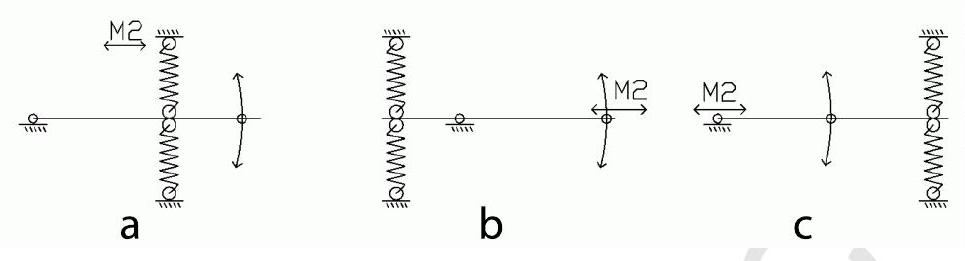
\includegraphics[width=\textwidth]{2025_09_17_f0417c8723605e4ad1efg-16}
\captionsetup{labelformat=empty}
\caption{Figure 7: Three possibilities of Controllable Transmission Ratio: a) changing spring, b) changing force, c) changing pivot point.}
\end{center}
\end{figure}

giving a lighter, more compact setup compared to the AwAS. CompAct ${ }^{(-}$ VSA is an improved version of AwAS II using a cam shaped lever arm with a variable pivot axis actuated by a rack and pinion transmission system [60]. The idea of changing the pivot point is also used in vsaUT-2 [61]. The stiffness change mechanism uses a ring gear, with pitch diameter d , and a pivot gear with pitch diameter $\mathrm{d} / 2$, to which the pivot point is connected. Due to the precise ratio between the pitch diameters, the pivot point moves in a straight line with respect to the ring gear when the pivot gear runs in the ring gear. Since the pivot moves in a straight line, no guides are needed, ensureing low friction when moving the pivot point. This concept is used in the mVSA-UT [62], which is actuated by differentially connected two motors, responsible for changing both the output stiffness and position. More specifically, in its realization, the output stiffness can vary from zero to almost infinite by moving the pivot point along the lever arm and the output shaft can perform unbounded and continuous rotations.

\subsection*{3.4.2. Nonlinear mechanical interlink}
By changing the properties of the mechanical interlink one can obtain different transmission ratios. In this category no devices have been reported in literature that use this as the primary principle to adapt the stiffness. However different connections principles exist to yield torque-deflection characteristics in function of the application (see Fig. 8).

Mostly the compliant elements are connected to the joint using a pulley (see Fig. 8a). PAMs for example have a limited joint motion due to the limited contraction ratio of the muscles and by choosing different connection principles the torque characteristic can be adjusted. In the biped Lucy [63] and the manipulator arm [64] a pull rod and leverage mechanism are implemented (see Fig. 8b). By changing the angle and length of the lever arms

\begin{figure}[h]
\begin{center}
  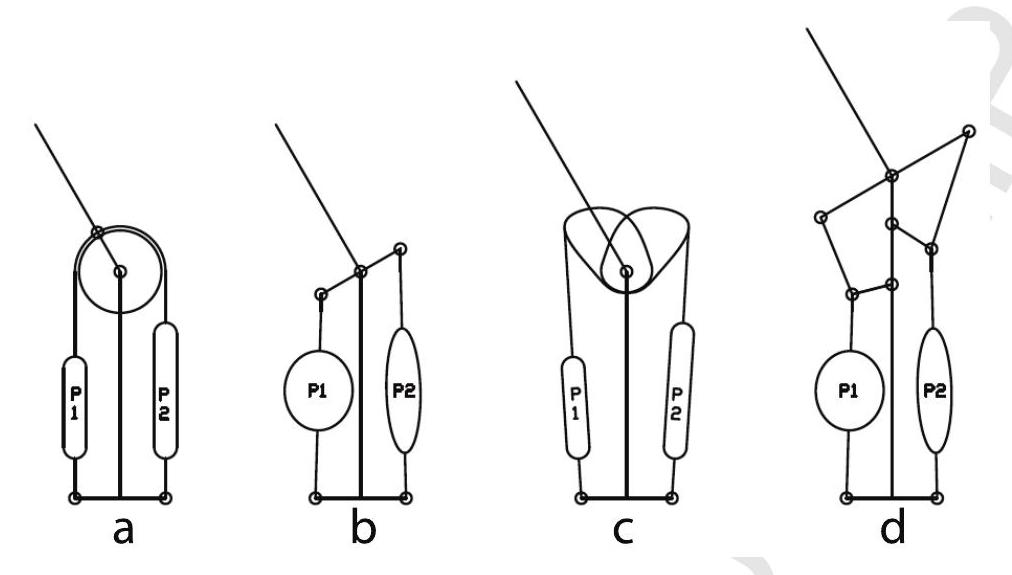
\includegraphics[width=\textwidth]{2025_09_17_f0417c8723605e4ad1efg-17}
\captionsetup{labelformat=empty}
\caption{Figure 8: Different connection principles: a ) pulley, b) pull rod mechanism, c) cam profile, d) four-bar mechanism).}
\end{center}
\end{figure}

the strong nonlinearity of the force-angle characteristic of the muscles is compensated in order to flatten the torque-angle characteristics of the joint. The knee rehabilitation robot Knexo uses a four-bar mechanism (see Fig. 8d) in order to be able to encapsulate the desired torque and joint range requirements with a relative simple and compact mechanism. Another advantage is that the coupler of each four-bar linkage is easily equipped with two pairs of strain gauges for joint torque measurements. An exhaustive search approach is proposed by Beyl et al. [65] to solve this multi-objective optimization problem. Shin et al. [66] developed a design methodology to synthesize a pair of variable radius pulleys (see Fig. 8c) that maintains high torque capacity while satisfying passive stiffness and workspace requirements.

In the VS-joint [55], Maccepa 2.0 [67] and FSJ [55] a cam profile is used to have a desired torque-deflection characteristic.

\subsection*{3.4.3. Continuously variable transmission}
A final approach in this class is continuously variable transmissions incorporating designs such as Variable-diameter pulleys (VDP) or Reeves drives, Toroidal or roller-based continuously variable transmission (CVT) and Magnetic CVTs [68]. Stramigioli et al. [27] proposed the use of infinitely variable transmissions (IVT), in which the gearing includes a zero ratio and also a negative ratio. This IVT is between the output link and the spring element (see Section 3.1.1). This actuator could be controlled differently without an engagement of the clutch, by controlling the rest position with the motor on\\
the other side of the spring and the stiffness with the adjustment of the IVT. The crucial element of this design is the IVT. A prototype has been built but not yet reported in the literature.

\subsection*{3.5. Physical properties of spring}
Unlike the previous concepts, structure control modulates the effective physical structure of a spring to achieve variations in stiffness. To understand the basic concept consider the basic elasticity law:


\begin{equation*}
F=\frac{E \cdot A}{L_{0}} \Delta L=K \Delta L \tag{1}
\end{equation*}


F is the force, E the material modulus, A the cross-sectional area, L the effective beam length, and $\Delta L$ is the extension. In this representation, $\mathrm{EA} / \mathrm{L}$ represents the stiffness K. To control the structural stiffness, any of the three parameters in this equation can be manipulated.

E is a material property, which cannot be controlled by a structural change, but for some materials, it can be changed e.g. by changing the temperature. Unfortunately these changes are not sufficiently rapid and there are no known VIA actuator examples.. Mechanisms where the cross section area A and the length of the elastic element L are changed, are discussed in the following sections.

\subsection*{3.5.1. Cross section area}
One technique to alter the cross section is to use a beam with non-unity aspect ratio where stiffness can be changed by rotating the beam through $90^{\circ}$ since the moment of inertia in the Bernoulli-Bar equation is the analogy to the cross section area. A prototype of a spring with variable stiffness is used in wearable robotic orthoses [69]. The helical spring in this design reduces the changes of lateral buckling. This is a simple way to obtain a compliant element with two predefined stiffness settings. To use such a device in an intermediate setting, solutions to the lateral buckling problem must be obtained. Seki et al. [70] used the rotated leaf spring approach, although they did not account for beam deflections beyond $15^{\circ}$ nor did they address the limitations due to lateral buckling. Kawamur et al. [70] changed the moment of inertia by controlling the force to press together an element consisting of many layered sheets. However, if the sheets are firmly pressed together, they will not slip due to friction. As a result, the element stiffens and larger forces are needed to bend the element. The forces can be electrostatic [71] or\\[0pt]
vacuum [70]. Note that holding the sheets together is very difficult because the shear forces are very high, but this system does benefit from simple construction and a wide stiffness range, although friction makes precise control of the stiffness difficult. Moreover, the stiffness will depend on the deflection when the volume is in a vacuum applied state.

\subsection*{3.5.2. Active spring length}
Stiffness may also be adjusted by varying the effective length of a compliant element. An active knee brace varies the beam length to adjust the stiffness [69]. The Mechanical Impedance Adjuster [72] contains a leaf spring, connected to the joint by a wire and a pulley. The effective length of the spring can be changed by a slider, with a roller on the slider holding the leaf spring close to the structure. The motor rotates the feed screw, which moves the slider, and thus changes the stiffness. A rotational version was implemented in a robotic joint. The two spindles, which are actuated by a motor, can move the slider with four wheels, rolling over the leaf spring to vary its effective length. An advantage of both of these mechanisms is that they are easy to construct and easy to control since the stiffness setting and equilibrium position are completely independent. This mechanism allows all possible states between compliant and very stiff.

An advantage of both of these mechanisms is that they are easy to construct and easy to control since the stiffness setting and equilibrium position are completely independent. This mechanism allows all possible states between compliant and very stiff.

Choi et al. [73] presented a variation of this method. The effective length of four springs split at $90^{\circ}$ around an axis were changed by moving the pivot, which had rollers sliding on the spring. The pivots were moved with a fourbar linkage. Controlling the two adjacent bars together in opposite direction, the pivot moved along the spring causing a stiffness change. When the bars rotated at the same speed in the same direction, the axis rotates without stiffness change but with change of equilibrium position.

Sugano et al. [74] designed a finger that incorporates a leaf spring that can be adjusted to vary the stiffness. The joint was not mounted rigidly but could move according to the stiffness of the leaf spring. De and Tasch designed a two dof degree-of-freedom finger, which again uses leaf springs, but can also control the coupling stiffness [75]. In [76] a torsional elastic element with a relocatable counter bearing changes the active spring length.

Stiffness adjustment in the Jack Spring is achieved by in/decreasing the

\begin{table}[h]
\begin{center}
\begin{tabular}{|l|l|l|l|l|l|l|l|l|}
\hline
\multirow{3}{*}{} & \multicolumn{8}{|c|}{adaptable compliance properties} \\
\hline
 & \multicolumn{3}{|c|}{spring preload} & \multicolumn{2}{|c|}{changing transmission load <-> spring} & \multicolumn{3}{|c|}{physical properties of spring} \\
\hline
 & preload adjustment of single spring & antagonistic springs with independent motors & antagonistic springs with antagonistic motors & lever length & continuously variable transmission & elasticity modus & cross section area & active spring length \\
\hline
Number of spring required & 1 & 2 & 2 & (1)2* & 1 & 1 & 1 & 1 \\
\hline
Can linear springs be used & yes & no & no & yes & yes & yes & yes & yes \\
\hline
Full energy capacity springs available at output & no & no & no & no & yes & yes & yes & no \\
\hline
Preload/pretension in equilibrium position & yes & yes & yes & no & no & no & no & no \\
\hline
Energy required to change stiffness at equilibrium position & yes & yes & yes & no & no & no & no & no \\
\hline
Completely stiff setting possible & no & no & no & yes & no & no & no & yes \\
\hline
Independent control stiffness and equilibrium position & yes & yes & no & yes & yes & yes & yes & yes \\
\hline
Possibility to design stiffness curve & yes & yes & yes & no & no & no & no & no \\
\hline
Passive deflection angle & large & medium & medium & small & large & large & large & medium \\
\hline
Active position range & large & large & small & large & large & large & large & large \\
\hline
Maximum torque equals max torque equilibrium position motor(s) & yes & no ** & no & yes & yes & yes & yes & yes \\
\hline
\end{tabular}
\captionsetup{labelformat=empty}
\caption{Figure 9: Overview of general properties variable stiffness actuators.}
\end{center}
\end{table}

\begin{itemize}
  \item in theory one spring that works in flexion-extension sufficient, in practice realised with two springs antagonistically placed\\
** in bi-directional arrangement the two motor torques add, at the loss of stiffness control\\[0pt]
number of coils used in a spring through a rotation of either the spring or the shaft/nut [77].
\end{itemize}

\subsection*{3.5.3. Comparison}
Comparing the different designs is quite difficult and is strongly dependent on the application. Therefore VIA-datasheet (presented in a follow-up paper [2]) were designed to compare quantitatively different designs. However, some general conclusions for the different classes and subclasses, are summarized in Fig. 9.

\section*{4. Inherent damping}
Inherently compliant actuators do have drawbacks: the mechanical resonance is decreased, compromising achievable bandwidth [78] [79] [80] [81]. The introduction of two complex conjugate poles also creates a sharp increase in phase lag, decreasing the stability margin when controlling the joint for link quantities and making the control difficult on the motor side due to the introduction of an anti-resonance at the same frequency. This creates problems particularly in the position/velocity control of such actuators at frequencies well below the mechanical resonance imposed by the compliance

\begin{figure}[h]
\begin{center}
  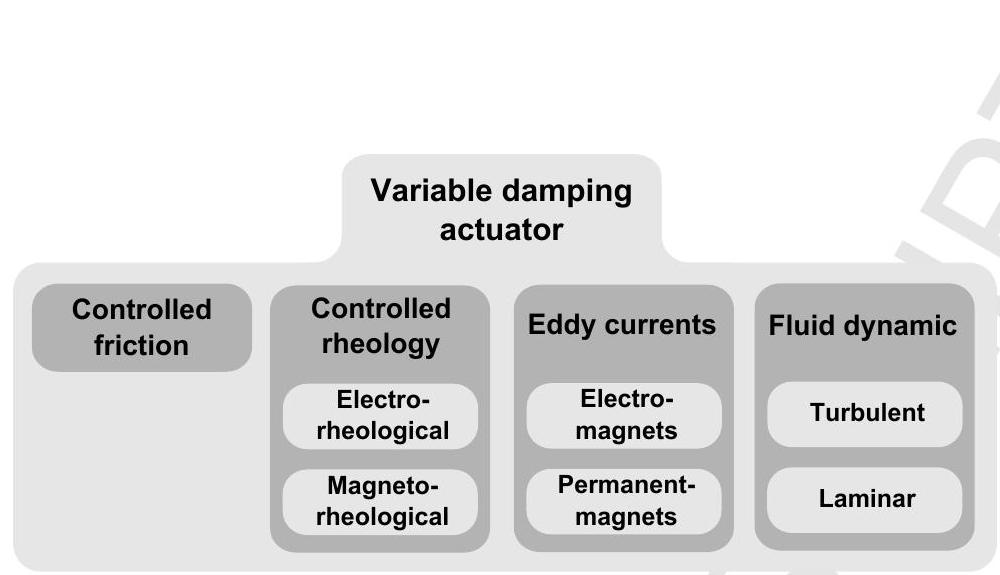
\includegraphics[width=\textwidth]{2025_09_17_f0417c8723605e4ad1efg-21}
\captionsetup{labelformat=empty}
\caption{Figure 10: Overview Inherent Damping Actuators}
\end{center}
\end{figure}

[82]. Furthermore, the induced underdamped oscillatory modes reduce the achievable performance of the position/velocity control. These oscillations may be suppressed by active damping control if the actuator dynamics are sufficiently high, however the resulting system would require a substantial amount of energy to accomplish such a highly dynamic task.

Inherent damping devices (fixed damping actuators and variable damping actuators) are designed to control robotic joints by providing physical damping. The Series Damper Actuator (SDA) [83], is a fixed damping actuator which uses a viscous damper between the actuator and the load. Twentyone has a torsion bar as an elastic element and a rotary damper around the bar as a pseudo damper [84]. Dampers have been thoroughly studied and have many different operating principles (Fig. 11). The most relevant are discussed here and displayed in Fig. 4.

\subsection*{4.1. Friction damper}
A Friction Damper (FD) is composed of an actuator that applies a normal force, $F_{n}$, on the output shaft (see Fig. 11a). A frictional damping force $F_{d}$ is produced as a consequence of relative motion. Because of the relative motion, a frictional damping force $F_{d}$ is produced as a consequence of the relative motion, and described by:


\begin{equation*}
F_{d}=-f F_{n} \operatorname{sign}\left(\dot{q}_{r}\right), \tag{2}
\end{equation*}


where $f$ is the friction coefficient and $\dot{q}_{r}$ the relative speed between the actuator and the output shaft. A more complex and realistic mathematical model can be found in [85]. Pure dry or lubricated friction is of no practical use because constant levels of friction can be optimized for a specific\\[0pt]
task however if the system has nonlinear dynamics or task variability (this is quite common in robotics systems) the global system performance might be deteriorated. If, however, the friction is modulated the performance can be improved. The challenge is therefore the control of the friction to obtain the desired damping characteristics. If the friction damper is properly controlled it can emulate viscous characteristics or any other type of nonlinear damping. It is also interesting to notice that this type of dampers can produce high damping forces at low velocities. Drawbacks of FD, pointed out in [85], are hysteresis and the presence of a static friction band [86] that can cause irregular behavior.

This principle has been used in [80] and [79] where three piezo stacks connected in parallel apply a braking force between two contact surfaces. This configuration demonstrates low energy consumption while being small, lightweight and clean. CompAct ${ }^{\text {® }}$ [80] combines the piezoelectric-based friction damper with a series elastic actuator of [21] marginally increasing the volume, without affecting the total length. Multidisc brakes actuated by electric motors have been tested in [87] and [88] uses magnetic particle \href{http://brakes.In}{brakes.In} [90] a powder brake was used for haptic rendering at high force bandwidth and magnitude. A Hot-Melt-Adhesive (HMA) as implemented in [89] exhibits visco-elastic characteristics that can reversibly change phase from solid to plastic to liquid.

\subsection*{4.2. Electrorheological and Magnetorheological Dampers}
Electrorheological (ER) and magnetorheological (MR) dampers (Fig. 11b) use liquids (Bingham fluids) whose viscosity depends on the electric or magnetic field strength respectively [86]. The property that can be changed is the yield stress itself.

The behavior of ER and MR fluids is given using Bingham viscoplastic models:


\begin{equation*}
F_{d}=-\operatorname{sign}\left(\dot{q}_{r}\right)\left(g\left(\mu,\left|\dot{q}_{r}\right|\right)+C u\right) \tag{3}
\end{equation*}


where $g\left(\mu,\left|\dot{q}_{r}\right|\right)$ represents the viscous component of the damping force, $\mu$ the viscosity of the fluid, $u$ the electric field or the current for ER and MR respectively and $C$ denotes a coefficient that depends on the physical properties of the fluid and on the geometry of the damper. The MR operating principle is often used to realize VDAs in robotics [90] [91] [83] [92] and also in vehicles [93] [94]. A more accurate model and a comparison between MR and FD can be found in [85], where it is pointed out that MR dampers, like the FDs, present high hysteresis.

\subsection*{4.3. Eddy Current Dampers}
Eddy Current Dampers (ECDs, see Fig. 11d) are magnetic devices composed of a conductive material moving through a magnetic field. Eddy currents are induced and create a damping force that is proportional to the relative velocity $\dot{q}_{r}$ between the material and the magnetic field:


\begin{equation*}
F_{d}=-D(r, d, h, B, \sigma) \dot{q}_{r} \tag{4}
\end{equation*}


The coefficient $D$ depends, ultimately, on the geometry of the conductor, represented by $r$, and of the magnet, denoted by $d$, their gap, $h$, the magnetic flux, $B$ and the specific conductivity of the conductor $\sigma$.

These devices can be realized with both permanent magnets or electromagnets. In both cases there is the possibility to design a device whose damping can be adjusted [95] [96] [97] [98]. In one case, the damping coefficient can be controlled by varying the intensity of the magnetic field, in the other case, by modifying the geometry of the conductor, or the gap between the conductor and the magnets (the effectiveness is shown in [97]). Albeit electromagnetic ECD are not composed of mobile parts, they have the disadvantage of consuming power while maintaining a fixed damping value.

This class of devices, being fluid-free and contact-free, is not affected by typical troubles due to oil (e.g., the need of seals against leakage), and by frictional wear. Still, they present the disadvantage of requiring a gearbox because of their low damping torque.

\subsection*{4.4. Fluid dynamics damper}
Two main possibilities exist when using fluids to damp: the quadratic damping (see Fig. 11c) and the linear damping (see Fig. 11e). The Reynolds number can be used as indicator of the main phenomenon by which the damper works. These two possibilities are described as follows:

\begin{itemize}
  \item when the fluid is characterized by turbulent flow (high Reynolds number) it produces a damping force proportional to the square of the relative speed
\end{itemize}


\begin{equation*}
F_{d}=-\operatorname{sign}\left(\dot{q}_{r}\right) C_{v} \dot{q}_{r}^{2} \tag{5}
\end{equation*}


from where the term quadratic damping comes from. A practical example of quadratic damping is a damper with an orifice allowing fluid flow, as largely used in automotive industry. Such device generates, at

\begin{figure}[h]
\begin{center}
  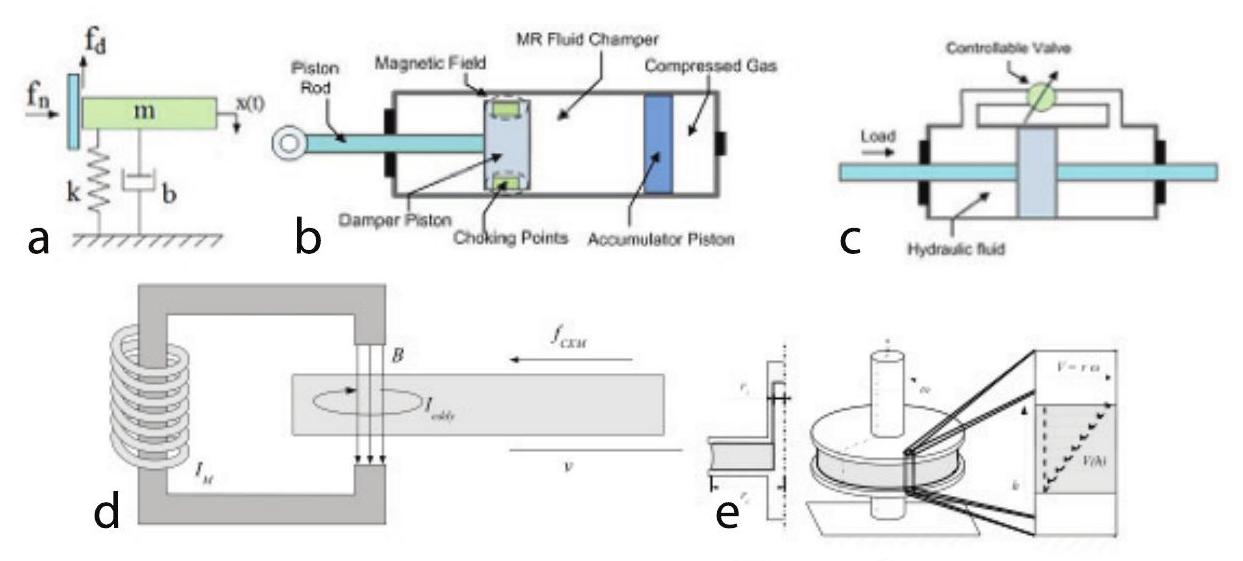
\includegraphics[width=\textwidth]{2025_09_17_f0417c8723605e4ad1efg-24}
\captionsetup{labelformat=empty}
\caption{Figure 11: Different variable damping actuator principles: a) friction, b) MR, c) variable Orifice fluid damper, d) eddy current, e) laminar viscous damping.}
\end{center}
\end{figure}

a given frequency, high damping for high amplitudes, but lower damping for lower amplitudes, and thus, has the drawback of presenting long lasting residual oscillations [86].

\begin{itemize}
  \item linear damping is the phenomenon present when a fluid is characterized by laminar flow (low Reynolds number) and produces a damping force proportional to the speed gradient in the fluid.
\end{itemize}


\begin{equation*}
F_{d}=-d(\mu, A, h) \dot{q}_{r} . \tag{6}
\end{equation*}


Here, the damping coefficient $d$ mainly depends on three parameters: $A$ the area of the surface in contact with the fluid; $h$ the height of the fluid chamber; and $\mu$, the viscosity of the fluid. Catalano et al. [99] implemented the control of the contact area $A$ by an aperture mechanism, similar to the light shutter of a camera, to engage a rotating chamber of high-viscosity silicon oil.

\section*{5. Combinations of inherent compliance and damping}
Some devices combine a variable damping actuator with an elastic element. To give an overview of the different possibilities consider a system described by: 1) one motor with an output shaft, 2) one containment frame, 3) one elastic connection between the motor and the shaft, and 4) one source of damping action. Since the list of system topologies grows exponentially\\
with the number of elements considered, we limit our analysis to systems composed of those four elements only. This gives rise to the four possible configurations shown in Fig. 12. Note that the damping action, represented with a pure damper in Fig. 12, could also be implemented with a hybrid visco-elastic element, this would imply slight modifications to equations 7-10. In this section we present an accurate analysis of these connection topologies and highlight benefits and drawbacks of each solution.

The topology depicted in Fig. 12(a) shows a stiffness and a damper in parallel between the reference and the link. The link dynamics of this layout is described by


\begin{equation*}
m \ddot{q}+d(\dot{q}-\dot{\theta})+k(q-\theta)=0 \tag{7}
\end{equation*}


where $m$ represents the link inertia, $d$ the damping, $k$ the stiffness, $q$ the link position, $\theta$ the reference position. This scheme has been considered in [100].

The scheme depicted in Fig. 12(b) presents a stiffness between the reference and the link, and a damper between the link and the external frame. The link dynamics of this layout is described by


\begin{equation*}
m \ddot{q}+d(\dot{q})+k(q-\theta)=0 . \tag{8}
\end{equation*}


This topology is featured, for example, in models of corresponding to a model of human limb impedance at a joint [101]. One drawback of system (b) is

\begin{figure}[h]
\begin{center}
  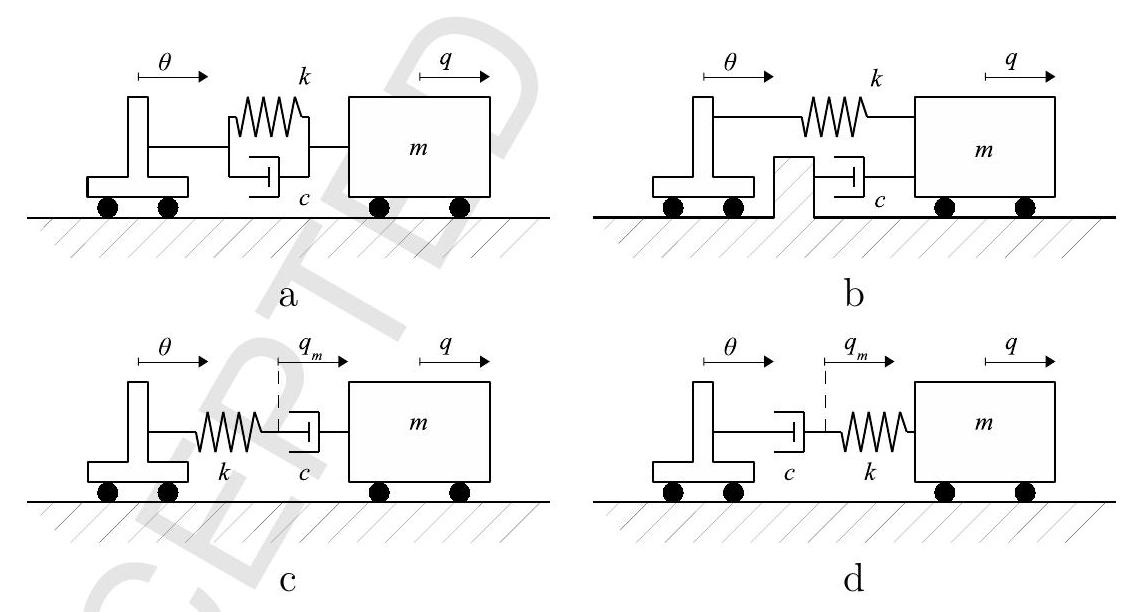
\includegraphics[width=\textwidth]{2025_09_17_f0417c8723605e4ad1efg-25}
\captionsetup{labelformat=empty}
\caption{Figure 12: The four possible layouts to add a damping action to a system coupling a motor with a load through an elastic connection: a) pure parallel, b) external parallel, c) serial spring first and d) serial damper first. The damping action can be introduced trough a pure damper, as shown in the figure, or with visco-elastic elements. More complex layouts are possible if a larger number of components is considered.}
\end{center}
\end{figure}

that, during link motion, the damper resistance must be overcome. This can be done by realizing a variable damping mechanism that can be completely turned off. On the other side, this system has the advantage of allowing the designer to realize it as an add on which can be attached externally to another actuation unit. This has been done using the variable fluid damping device of Catalano et al. [99], which is combined with the Qbot module [102]. Radulescu et al. [103] proposed the Maccepa-VD (Maccepa with Variable Damping) where the damper is a back-drivable motor/gearbox that exploits the DC motor damping effect. It is not the like in system (a), which has to be integrated into the device.

Schemes in Fig. 12(c) and (d) present a serial connection of a spring and a damper between the reference and the link. The link dynamics of these layouts are described by


\begin{gather*}
m \ddot{q}+d\left(\dot{q}-\dot{q}_{m}\right)=0 \\
d\left(\dot{q}_{m}-\dot{q}\right)+k\left(q_{m}-\theta\right)=0 \tag{9}
\end{gather*}


and


\begin{gather*}
m \ddot{q}+k\left(q-q_{m}\right)=0 \\
d\left(\dot{q}_{m}-\dot{\theta}\right)+k\left(q_{m}-q\right)=0 \tag{10}
\end{gather*}


respectively. These two schemes are similar to those adopted in [96] and [83] and present the advantage of minimizing the amount of motor inertia reflected to the link. Nevertheless, they have the major disadvantage of requiring continuous rotation of the motor to apply a constant torque to the output.

Some other differences arise between the four schemes, for instance, to achieve the behavior of a pure VSA, the damping factor should be null for layouts (a) and (b), while it should tend to infinity for layouts (c) and (d).

\section*{6. Inertial actuators}
Since impedance is defined as the differential operator relating the time course of reaction force $\mathrm{F}(\mathrm{t})$ to the time course of position ( $\mathrm{P}(\mathrm{t})$, the impedance of a inertia $M$ is (in the Laplace domain for simplicity):


\begin{equation*}
I(s)=\frac{F(s)}{P(s)}=\frac{1}{M s^{2}} \tag{11}
\end{equation*}


So a mass can also be used as a storage of kinetic energy apart from a spring and damper. For example in a hammer kinetic energy can be accumulated to drive a nail in a piece of wood [104]. A spinning flywheel is employed to act as a gyroscope to stabilize the robot and it can be steered by tilting [105] or used to store and release rotational energy for example used in the vehicles as Formula 1 [106]. Modulation of the impedance can be achieved by for example a variable transmission.

\section*{7. Conclusion}
Variable Impedance Actuators are under investigation to achieve safe, energy-efficient, and highly dynamic motion for powering the next generation of robots which have to collaborate with humans and interact with an unknown environment. The advances in VIA technology will pave the way towards new application fields, such as industrial co-workers, household robots, advanced prostheses and rehabilitation devices, and autonomous robots for exploration of space and hostile environments.

This paper presented an overview of the different variable impedance actuators developed so far, and proposes a classification based on how the variable stiffness and damping are achieved. The main classes are active impedance by control, inherent compliance and damping actuators, inertial and combinations of them. This classification allows for designer of new devices to orientate and take inspiration and users of VIA's to be guided in the design and implementation process for their targeted application. Datasheets with motor specifications are important tools in the design process, but yet unavailable for VIA's. The VIACTORS consortium has come up with a proposal for a VIA-datasheet which will be presented in a follow-up paper [2]. Designer's Guidelines for designing new VSA systems and their typical use-cases are discussed in [3].

\section*{8. Acknowledgments}
This work has been funded by the European Commissions 7th Framework Program as part of the project VIACTORS under grant no. 231554. From the second name, the authors are in alphabetical order.\\[0pt]
[1] A. Albu-Schaeffer, A. Bicchi, S. Stramigioli, E. Burdet, P. Smagt, A. Parravicini, D. Lefeber, N. Tsagarakis, VIACTORS-Variable

Impedance ACTuation systems embodying advanced interaction behaviors, in: European Future Technologies Conference (FET09), 2009.\\[0pt]
[2] G. Grioli, M. Garabini, M. Catalano, M. Mancini, B. Vanderborght, S. Wolf, M. Grebenstein, W. Friedl, M. Laffranchi, R. Carloni, R. V. Ham, E. Burdet, D. Lefeber, D. Caldwell, N. Tsagarakis, S. Stramigioli, A. Albu-Schaeffer, A. Bicchi, Variable stiffness actuators: the user's point of view., IEEE Robotics and Automation Magazine (under review).\\[0pt]
[3] S. Wolf, G. Grioli, M. Garabini, M. Catalano, M. Mancini, B. Vanderborght, M. Grebenstein, W. Friedl, M. Laffranchi, R. Carloni, R. V. Ham, E. Burdetk, D. Lefeber, D. Caldwell, N. Tsagarakis, S. Stramigioli, A. Albu-Schaeffer, A. Bicchi, Variable stiffness actuators: Design and components, IEEE Robotics and Automation Magazine (under review).\\[0pt]
[4] K. Salisbury, B. Eberman, M. Levin, W. Townsend, The design and control of an experimental whole-arm manipulator, in: The fifth international symposium on Robotics research, MIT Press, 1991, pp. 233-241.\\[0pt]
[5] N. Hogan, Impedance control: An approach to manipulation: Part Ill - applications, Journal of dynamic systems, measurement, and control 107 (2) (1985) 17.\\[0pt]
[6] H. Asada, K. Youcef-Toumi, Direct-drive robots: theory and practice, MIT Press, 1987.\\[0pt]
[7] R. Pfeifer, J. Bongard, S. Grand, How the body shapes the way we think: a new view of intelligence, The MIT Press, 2007.\\[0pt]
[8] J. E. Colgate, N. Hogan, Robust control of dynamically interacting systems, International journal of Control 48 (1) (1988) 65-88.\\[0pt]
[9] V. Duindam, A. Macchelli, S. Stramigioli, H. Bruyninckx, Modeling and Control of Complex Physical Systems: The Port-Hamiltonian Approach, Springer, 2009.\\[0pt]
[10] B. Vanderborght, A. Albu-Schaeffer, A. Bicchi, E. Burdet, D. Caldwell, R. Carloni, M. Catalano, G. Ganesh, M. Garabini, G. Grioli,\\
S. Haddadin, A. Jafari, M. Laffranchi, D. Lefeber, F. Petit, S. Stramigioli, M. Grebenstein, N. Tsagarakis, M. Van Damme, R. Van Ham, L. Visser, S. Wolf, Variable impedance actuators: Moving the robots of tomorrow, in: IEEE/RSJ International Conference on Intelligent Robots and Systems (IROS 2012), 2012.\\[0pt]
[11] R. Van Ham, S. Thomas, B. Vanderborght, K. Hollander, D. Lefeber, Compliant actuator designs: Review of actuators with passive adjustable compliance/controllable stiffness for robotic applications, IEEE Robotics and Automation Magazine 16 (3) (2009) 81-94.\\[0pt]
[12] A. Albu-Schaffer, S. Haddadin, C. Ott, A. Stemmer, T. Wimbock, G. Hirzinger, The DLR lightweight robot: design and control concepts for robots in human environments, Industrial Robot: An International Journal 34 (5) (2007) 376-385.\\[0pt]
[13] J. Pratt, Exploiting inherent robustness and natural dynamics in the control of bipedal walking robots, Ph.D. thesis, Massachusetts Institute of Technology (2000).\\[0pt]
[14] R. Bischoff, J. Kurth, G. Schreiber, R. Koeppe, A. Albu-Schäffer, A. Beyer, O. Eiberger, S. Haddadin, A. Stemmer, G. Grunwald, et al., The KUKA-DLR lightweight robot arm-a new reference platform for robotics research and manufacturing, in: 6th German Conference on Robotics (ROBOTIK), VDE, 2010, pp. 1-8.\\[0pt]
[15] T. Boaventura, C. Semini, J. Buchli, M. Frigerio, M. Focchi, D. G. Caldwell, Dynamic torque control of a hydraulic quadruped robot, in: IEEE International Conference on Robotics and Automation (ICRA), IEEE, 2012, pp. 1889-1894.\\[0pt]
[16] S.-H. Hyon, J. G. Hale, G. Cheng, Full-body compliant humanhumanoid interaction: balancing in the presence of unknown external forces, IEEE Transactions on Robotics 23 (5) (2007) 884-898.\\[0pt]
[17] E. D. Fasse, N. Hogan, S. R. Gomez, N. R. Mehta, A novel variable mechanical impedance electromechanical actuator, Dynamic Systems and Control 55 (1) (1994) 311-318.\\[0pt]
[18] F. Petit, A. Albu-Schaffer, State feedback damping control for a multi DOF variable stiffness robot arms, in: IEEE International Conference on Robotics and Automation (ICRA 2011), 2011, pp. 5561-5567.\\[0pt]
[19] G. Pratt, M. Williamson, Series elastic actuators, in: IEEE International Workshop on Intelligent Robots and Systems (IROS 1990), 1990, pp. 399-406.\\[0pt]
[20] T. Sugar, A novel selective compliant actuator, Mechatronics 12 (9) (2002) 1157-1171.\\[0pt]
[21] N. Tsagarakis, M. Laffranchi, B. Vanderborght, D. Caldwell, A Compact Soft Actuator Unit for Small Scale Human Friendly Robots, in: IEEE International Conference on Robotics and Automation (ICRA 2009), 2009, pp. 4356-4362.\\[0pt]
[22] M. Zinn, O. Khatib, B. Roth, J. Salisbury, Playing it safe [humanfriendly robots], IEEE Robotics \& Automation Magazine 11 (2) (2004) 12-21.\\[0pt]
[23] D. Shin, I. Sardellitti, Y. Park, O. Khatib, M. Cutkosky, Design and control of a bio-inspired human-friendly robot, The International Journal of Robotics Research 29 (5) (2010) 571-584.\\[0pt]
[24] A. Seyfarth, H. Geyer, R. Blickhan, S. Lipfert, J. Rummel, Y. Minekawa, F. Iida., Fast Motions in Biomechanics and Robotics, Vol. 340, Springer Berlin / Heidelberg, 2006, Ch. Running and walking with compliant legs, pp. 383-401.\\[0pt]
[25] I. Thorson, D. G. Caldwell, A nonlinear series elastic actuator for highly dynamic motions, in: IEEE/RSJ International Conference on Intelligent Robots and Systems (IROS 2011), 2011, pp. 390-394.\\[0pt]
[26] J. Park, B. Kim, J. Song, H. Kim, Safe link mechanism based on nonlinear stiffness for collision safety, Mechanism and Machine Theory 43 (10) (2008) 1332-1348.\\[0pt]
[27] S. Stramigioli, G. van Oort, E. Dertien, A concept for a new energy efficient actuator, in: IEEE/ASME International Conference on Advanced Intelligent Mechatronics (AIM 2008), 2008, pp. 671-675.\\[0pt]
[28] N. Hogan, Adaptive control of mechanical impedance by coactivation of antagonist muscles, IEEE Transactions on Automatic Control 29 (8) (1984) 681-690.\\[0pt]
[29] B. Verrelst, R. Van Ham, B. Vanderborght, D. Lefeber, F. Daerden, M. Van Damme, Second generation pleated pneumatic artificial muscle and its robotic applications, Advanced Robotics 20 (7) (2006) 783-805.\\[0pt]
[30] G. Tonietti, R. Schiavi, A. Bicchi, Design and control of a variable stiffness actuator for safe and fast physical human/robot interaction, in: IEEE International Conference on Robotics and Automation (ICRA 2005), 2005, pp. 526-531.\\[0pt]
[31] R. Schiavi, G. Grioli, S. Sen, A. Bicchi, VSA-II: A novel prototype of variable stiffness actuator for safe and performing robots interacting with humans, in: IEEE International Conference on Robotics and Automation (ICRA 2008), 2008, pp. 2171-2176.\\[0pt]
[32] M. Catalano, G. Grioli, M. Garabini, F. Bonomo, M. Mancini, N. Tsagarakis, A. Bicchi, VSA-CubeBot: a modular variable stiffness platform for multiple degrees of freedom robots., IEEE International Conference on Robotics and Automation (ICRA 2011) (2011) 5090 5095.\\[0pt]
[33] S. Wolf, G. Hirzinger, A new variable stiffness design: Matching requirements of the next robot generation, in: IEEE International Conference on Robotics and Automation (ICRA 2008), 2008, pp. 17411746.\\[0pt]
[34] F. Petit, M. Chalon, W. Friedl, M. Grebenstein, A. Albu-Schaeffer, G. Hirzinger, Bidirectional antagonistic variable stiffness actuation: Analysis, design and implementation, in: Proc. IEEE International Conf. on Robotics and Automation (ICRA 2010), 2010, pp. 4189-4196.\\[0pt]
[35] E. C. Martinez-Villalpando, H. Herr, Agonist-antagonist active knee prosthesis: A preliminary study in level-ground walking, J Rehabil Res Dev 46 (3) (2009) 361-73.\\[0pt]
[36] N. Vitiello, T. Lenzi, S. Roccella, S. M. M. De Rossi, E. Cattin, F. Giovacchini, F. Vecchi, M. C. Carrozza, Neuroexos: A powered elbow ex-\\
oskeleton for physical rehabilitation, IEEE Transactions on Robotics 29 (1) (2013) 220-235.\\[0pt]
[37] D. G. Caldwell, G. Medrano-Cerda, M. Goodwin, Control of pneumatic muscle actuators, IEEE Control Systems Magazine 15 (1) (1995) 40-48.\\[0pt]
[38] O. Eiberger, S. Haddadin, M. Weis, A. Albu-Schäffer, G. Hirzinger, On joint design with intrinsic variable compliance: Derivation of the DLR QA-Joint, in: IEEE International Conference on Robotics and Automation (ICRA 2010), 2010, pp. 1687-1694.\\[0pt]
[39] J. W. Hurst, A. A. Rizzi, Series compliance for robot actuation: Application on the electric cable differential leg, IEEE Robotics \& Automation Magazine 15 (3) (2008) 2008.\\[0pt]
[40] C. English, D. Russell, Mechanics and stiffness limitations of a variable stiffness actuator for use in prosthetic limbs, Mechanism and Machine Theory 34 (1) (1999) 7-25.\\[0pt]
[41] C. English, D. Russell, Implementation of variable joint stiffness through antagonistic actuation using rolamite springs, Mechanism and machine theory 34 (1) (1999) 27-40.\\[0pt]
[42] M. Grebenstein, P. van der Smagt, Antagonism for a highly anthropomorphic handarm system, Advanced Robotics 22 (1) (2008) 39-55.\\[0pt]
[43] M. Grebenstein, A. Albu-Schäffer, T. Bahls, M. Chalon, O. Eiberger, W. Friedl, R. Gruber, U. Hagn, R. Haslinger, H. Höppner, et al., The DLR hand arm system, in: International Conference on Robotics and Automation (ICRA 2011), Vol. 11, 2010.\\[0pt]
[44] T. Huang, J. Kuan, H. Huang, Design of a new variable stiffness actuator and application for assistive exercise control, in: IEEE/RSJ International Conference on Intelligent Robots and Systems (IROS 2011), IEEE, 2011, pp. 372-377.\\[0pt]
[45] B. Tondu, P. Lopez, Modeling and control of mckibben artificial muscle robot actuators, Control Systems Magazine, IEEE 20 (2) (2000) 15-38.\\[0pt]
[46] D. C. Villegas, M. Van Damme, B. Vanderborght, D. Lefeber, Third generation pleated pneumatic artificial muscles for robotic applications: Development and comparison with McKibben muscles, Advanced Robotics 26 (2012) 1205-1227.\\[0pt]
[47] M. Randazzo, M. Fumagalli, G. Metta, G. Sandini, Closed loop control of a rotational joint driven by two antagonistic dielectric elastomer actuators, in: Society of Photo-Optical Instrumentation Engineers (SPIE) Conference Series, Vol. 7642, 2010, p. 68.\\[0pt]
[48] F. Carpi, D. D. Rossi, R. Kornbluh, R. Pelrine, P. Sommer-Larsen (Eds.), Dielectric elastomers as electromechanical transducers: Fundamentals, materials, devices, models and applications of an emerging electroactive polymer technology, Oxford: Elsevier, 2008.\\[0pt]
[49] B. Vanderborght, T. Sugar, R. Van Ham, K. Hollander, D. Lefeber, Comparison of mechanical design and energy consumption of adaptable passive compliant actuators, International Journal of Robotics Research 28 (1) (2008) 90-103.\\[0pt]
[50] R. Carloni, L. C. Visser, S. Stramigioli, Variable stiffness actuators: A port-based power-flow analysis, IEEE Transactions on Robotics 28 (1).\\[0pt]
[51] R. Van Ham, B. Vanderborght, M. Van Damme, B. Verrelst, D. Lefeber, MACCEPA, the Mechanically Adjustable Compliance and Controllable Equilibrium Position Actuator: Design and Implementation in a Biped Robot, Robotics and Autonomous Systems 55 (10) (2007) 761-768.\\[0pt]
[52] J. Sulzer, M. Peshkin, J. Patton, MARIONET: An exotendon-driven, rotary series elastic actuator for exerting joint torque, in: International Conference on Robotics for Rehabilitation (ICORR 2005), 2005, pp. 103-108.\\[0pt]
[53] Y. Mao, J. Wang, P. Jia, S. Li, Z. Qiu, L. Zhang, Z. Han, A reinforcement learning based dynamic walking control, in: IEEE International Conference on Robotics and Automation (ICRA 2007), 2007, pp. 36093614.\\[0pt]
[54] D. Braun, M. Howard, S. Vijayakumar, Exploiting variable stiffness in explosive movement tasks, in: Robotics Science and Systems (RSS), 2011.\\[0pt]
[55] S. Wolf, O. Eiberger, G. Hirzinger, The DLR FSJ: Energy based design of a variable stiffness joints, in: IEEE International Conference on Robotics and Automation (ICRA 2011), 2011, pp. 5082-5089.\\[0pt]
[56] L. C. Visser, R. Carloni, S. Stramigioli, Energy efficient variable stiffness actuators, IEEE Transactions on Robotics 27 (5) (2011) 865-875.\\[0pt]
[57] A. Jafari, N. Tsagarakis, B. Vanderborght, D. Caldwell, A novel actuator with adjustable stiffness (AwAS), in: IEEE/RSJ International Conference on Intelligent Robots and Systems (IROS 2010), 2010, pp. 4201-4206.\\[0pt]
[58] B.-S. Kim, J.-B. Song, Design and control of a variable stiffness actuator based on adjustable moment arm, IEEE Transactions on Robotics 28 (5) (2012) 1145-1151.\\[0pt]
[59] A. Jafari, N. Tsagarakis, D. G. Caldwell, AwAS-II: A new actuator with adjustable stiffness based on the novel principle of adaptable pivot point and variable lever ratio, in: IEEE International Conference on Robotics and Automation (ICRA), 2011, pp. 4638-4643.\\[0pt]
[60] N. Tsagarakis, I. Sardellitti, C. D. G., A new variable stiffness actuator (CompAct-VSA): Design and modelling, 2011, pp. 378-383.\\[0pt]
[61] S. S. Groothuis, G. Rusticelli, A. Zucchelli, S. Stramigioli, R. Carloni, The vsaUT-II: a novel rotational variable stiffness actuator, in: IEEE International Conference on Robotics and Automation (ICRA 2012), 2012.\\[0pt]
[62] M. Fumagalli, E. Barrett, S. Stramigioli, R. Carloni, The mVSA-UT: a miniaturized differential mechanism for a continuous rotational variable stiffness actuator, in: 4th IEEE RAS \& EMBS International Conference on Biomedical Robotics and Biomechatronics (BioRob 2012), 2012, pp. 1943-1948.\\[0pt]
[63] B. Vanderborght, R. Van Ham, B. Verrelst, M. Van Damme, D. Lefeber, Overview of the lucy project: Dynamic stabilization of\\
a biped powered by pneumatic artificial muscles, Advanced Robotics 22 (25) (2008) 1027-1051.\\[0pt]
[64] M. Van Damme, B. Vanderborght, B. Verrelst, R. Van Ham, F. Daerden, D. Lefeber, Proxy-based sliding mode control of a planar pneumatic manipulator, International Journal of Robotics Research 28 (2) (2009) 266-284.\\[0pt]
[65] P. Beyl, M. Van Damme, R. Van Ham, B. Vanderborght, D. Lefeber, Design and control of a lower limb exoskeleton for robot-assisted gait training, Applied Bionics and Biomechanics 6 (2) (2009) 229-243.\\[0pt]
[66] D. Shin, X. Yeh, O. Khatib, Variable radius pulley design methodology for pneumatic artificial muscle-based antagonistic actuation systems, IEEE/RSJ International Conference on Intelligent Robots and Systems (IROS 2011) (2011) 1830-1835.\\[0pt]
[67] B. Vanderborght, N. Tsagarakis, R. Van Ham, I. Thorson, D. Caldwell, Maccepa 2.0: compliant actuator used for energy efficient hopping robot chobino1d, Autonomous Robots (2009) 1-11.\\[0pt]
[68] N. Sclater, Mechanisms and mechanical devices sourcebook, McGrawHill Professional, 2011.\\[0pt]
[69] K. Hollander, T. Sugar, Concepts for compliant actuation in wearable robotic systems, in: US-Korea Conference on Science, Technology and Entrepreneurship (UKC2004), 2004.\\[0pt]
[70] S. Kawamura, T. Yamamoto, D. Ishida, T. Ogata, Y. Nakayama, O. Tabata, S. Sugiyama, Development of passive elements with variable mechanical impedance for wearable robots, in: IEEE International Conference on Robotics and Automation (ICRA 2002), Vol. 1, 2002, pp. 248-253.\\[0pt]
[71] O. Tabata, S. Konishi, P. Cusin, Y. Ito, F. Kawai, S. Hirai, S. Kawamura, Microfabricated tunable bending stiffness device, in: The Thirteenth Annual International Conference on Micro Electro Mechanical Systems (MEMS 2000), 2000, pp. 23-27.\\[0pt]
[72] T. Morita, S. Sugano, Design and development of a new robot joint using a mechanical impedance adjuster, in: IEEE International Conference on Robotics and Automation (ICRA 1995), Vol. 3, 1995, pp. 2469-2475.\\[0pt]
[73] J. Choi, S. Hong, W. Lee, S. Kang, M. Kim, A robot joint with variable stiffness using leaf springs, IEEE Transactions on Robotics 27 (2) (2011) 229-238.\\[0pt]
[74] S. Sugano, S. Tsuto, I. Kato, Force control of the robot finger joint equipped with mechanical compliance adjuster, in: lEEE/RSJ International Conference on Intelligent Robots and Systems (IROS 1992), Vol. 3, 1992, pp. 2005-2013.\\[0pt]
[75] A. De, U. Tasch, A two-DOF manipulator with adjustable compliance capabilities and comparison with the human finger, in: Journal of Robotic System, Vol. 13, New York, NY: Wiley, c1984-c2005., 1996, pp. 25-34.\\[0pt]
[76] J. Schuy, P. Beckerle, J. Wojtusch, S. Rinderknecht, O. von Stryk, Conception and evaluation of a novel variable torsion stiffness for biomechanical applications, in: 4th IEEE RAS \& EMBS International Conference on Biomedical Robotics and Biomechatronics (BioRob), 2012, pp. 713-718.\\[0pt]
[77] K. Hollander, T. Sugar, D. Herring, Adjustable robotic tendon using a "jack spring" ${ }^{T M}$, in: 9th International Conference on Rehabilitation Robotics (ICORR 2005), 2005, pp. 113-118.\\[0pt]
[78] M. Laffranchi, N. G. Tsagarakis, D. G. Caldwell, Analysis and development of a semiactive damper for compliant actuation systems, IEEE/ASME Transactions on Mechatronics.\\[0pt]
[79] M. Laffranchi, N. Tsagarakis, A compact compliant actuator (CompAct ${ }^{\dagger M}$ ) with variable physical damping, in: IEEE International Conference on Robotics and Automation (ICRA 2011), 2011, pp. 4644-4650.\\[0pt]
[80] M. Laffranchi, N. Tsagarakis, D. Caldwell, A variable physical damping actuator (VPDA) for compliant robotic joints, IEEE International Conference on Robotics and Automation (ICRA 2010) (2010) 16681674.\\[0pt]
[81] J. Hurst, A. Rizzi, D. Hobbelen, Series elastic actuation: Potential and pitfalls, in: International Conference on Climbing and Walking Robots, 2004.\\[0pt]
[82] A. De Luca, W. Book, Robots with flexible elements, Handbook of Robotics, B. Siciliano and O. Khatib, Eds., Springer (2008) 287-319.\\[0pt]
[83] C. Chew, G. Hong, W. Zhou, Series damper actuator: a novel force/torque control actuator, in: 4th IEEE/RAS International Conference on Humanoid Robots, Vol. 2, 2004, pp. 533-546.\\[0pt]
[84] H. Iwata, S. Sugano, Design of human symbiotic robot TWENDYONE, in: IEEE International Conference on Robotics and Automation ICRA 2009), 2009, pp. 580-586.\\[0pt]
[85] E. Guglielmino, C. Stammers, K. Edge, Damp-by-wire: magnetorheological vs friction dampers', 16th IFAC World.\\[0pt]
[86] J. C. Dixon, The Shock Absorber Handbook, Senior Lecture in Engineering Mechanics, PEP and Wiley, 2007.\\[0pt]
[87] R. J. Farris, M. Goldfarb, Design of a multidisc electromechanical brake, IEEE/ASME Transactions on Mechatronics 16 (6) (2011) 985993.\\[0pt]
[88] M. R. Tucker, R. Gassert, Differential-damper topologies for actuators in rehabilitation robotics, in: Annual International Conference of Engineering in Medicine and Biology Society (EMBC 2012), 2012, pp. 3081-3085.\\[0pt]
[89] K. Gunura, J. Bocanegra, F. Iida, Design and control of a novel viscoelastic braking mechanism using HMA, Intelligent Robotics and Applications (2011) 416-425.\\[0pt]
[90] E. Garcia, J. Arevalo, F. Sanchez, J. Sarria, P. Gonzalez-de Santos, Design and development of a biomimetic leg using hybrid actuators, in: IEEE/RSJ International Conference on Intelligent Robots and Systems (IROS 2011), 2011, pp. 1507-1512.\\[0pt]
[91] D. Chapuis, R. Gassert, E. Burdet, H. Bleuler, A hybrid ultrasonic motor and electrorheological fluid clutch actuator for force-feedback in

MRI/fMRI, in: 30th Annual International Conference of the IEEE Engineering in Medicine and Biology Society (EMBS 2008), IEEE, 2008, pp. 3438-3442.\\[0pt]
[92] P. Fauteux, M. Lauria, B. Heintz, F. Michaud, Dual-differential rheological actuator for high-performance physical robotic interaction, IEEE Transactions on Robotics 26 (4) (2010) 607-618.\\[0pt]
[93] J. Li, D. Jin, X. Zhang, J. Zhang, W. Gruver, An electrorheological fluid damper for robots, in: IEEE International Conference on Robotics and Automation (ICRA 1995), 1995, pp. 2631-2636.\\[0pt]
[94] J. Desrosiers, J. L. Bigué, M. Denninger, G. Julió, J. Plante, F. Charron, Preliminary investigation of magneto-rheological fluid durability in continuous slippage clutch, in: Journal of Physics: Conference Series, Vol. 412, 2013, p. 012022.\\[0pt]
[95] B. Ebrahimi, M. B. Khamesee, F. Golnaraghi, A novel eddy current damper: theory and experiment, Journal of Physics D: Applied Physics 42 (7) (2009) 075001.\\[0pt]
[96] A. H. C. Gosline, V. Hayward, Eddy current brakes for haptic interfaces: Design, identification, and control, IEEE/ASME Transactions on Mechatronics 13 (6) (2008) 669-677.\\[0pt]
[97] H. A. Sodano, J.-S. Bae, D. Inman, K. Belvin, Improved concept and model of eddy current damper, Transaction of the ASME 128 (2006) 294-302.\\[0pt]
[98] A. Mohand-Ousaid, G. Millet, S. Régnier, S. Haliyo, V. Hayward, Haptic interface transparency achieved through viscous coupling, The International Journal of Robotics Research 31 (3) (2012) 319-329.\\[0pt]
[99] M. Catalano, G. Grioli, M. Garabini, F. W. Belo, A. di Basco, N. Tsagarakis, A. Bicchi, Implementing a variable impedance actuator, in: IEEE International Conference on Robotics and Automation (ICRA 2012), 2012.\\[0pt]
[100] N. G. Tsagarakis, M. Lafranchi, D. G. Caldwell, Developing actuators with rich motor properties for emerging humanoids, Proceedings of SIMPAR (2010) 113-125.\\[0pt]
[101] T. Milner, C. Cloutier, Compensation for mechanically unstable loading in voluntary wrist movement, Experimental Brain Research 94 (3) (1993) 522-532.\\[0pt]
[102] M. G. Catalano, G. Grioli, VSA-CubeBot: A modular variable stiffness platform for multiple degrees of freedom robots, in: IEEE International Conference on Robotics and Automation (ICRA 2011), 2011, pp. 50905095.\\[0pt]
[103] A. Radulescu, M. Howard, D. Braun, S. Vijayakumar, Exploiting variable physical damping in rapid movement tasks, in: IEEE/ASME International Conference on Advanced Intelligent Mechatronics (AIM 2012), 2012, pp. 141-148.\\[0pt]
[104] M. Garabini, A. Passaglia, F. Belo, P. Salaris, A. Bicchi, Optimality principles in variable stiffness control: The VSA hammer, in: IEEE/RSJ International Conference on Intelligent Robots and Systems (IROS 2011), 2011, pp. 3770-3775.\\[0pt]
[105] Y. Xu, S. Au, Stabilization and path following of a single wheel robot, IEEE/ASME Transactions on Mechatronics 9 (2) (2004) 407-419.\\[0pt]
[106] K. Pullen, C. Ellis, Kinetic energy storage for vehicles, in: Hybrid Vehicle Conference, IET The Institution of Engineering and Technology, 2006, IET, 2006, pp. 91-108.


\end{document}